\documentclass[a4paper,10pt,twocolumn,uplatex]{jsarticle}
\usepackage{style/nislab}

%---------------------------------------------------------------------
% レジュメ種別・日付設定(要変更)
% \type{} 1:修士論文諮問会 2:卒業論文発表会 else:月例発表会
\type{3}
\year{2021}
\month{8}
\date{13}

%---------------------------------------------------------------------
% ページ番号設定(要変更)
\setcounter{page}{3}

%---------------------------------------------------------------------
\begin{document}
%---------------------------------------------------------------------
% タイトル作成部分(要変更)
% \maketitle{タイトル}{title}{名前}{name}
\maketitle{SDNによるQoSを考慮したIoT通信制御手法}
{A Method of SDN Based QoS Aware IoT Communication Management}
{国本 典晟}
{Tensei Kunimoto}

%---------------------------------------------------------------------
\section{はじめに}
近年,画像や動画などの大容量データの需要が急速に拡大したことによるインターネット全体の帯域の逼迫が問題になっているが,IoTデバイスの増加とスマートホームの技術の進歩に伴い,ホームネットワーク内部の帯域並びにホームネットワーク外部のインターネットの帯域の逼迫はより深刻化すると予想される.現在,ISP (Internet Service Provider) は各家庭の総帯域を契約した帯域の範囲内で制御しており,要求される帯域が回線の帯域を上回る場合、特定アプリケーションやユーザの帯域を制御することでネットワークの品質確保に努めている\cite{guideline}.しかし,そういった帯域制御は多様なサービスやトラフィックに最適化されたものではなく,IoTデバイスが要求する複数のQoS要件を満たすことができない.\par
この問題の解決

%---------------------------------------------------------------------
\section{関連研究}

%---------------------------------------------------------------------
\subsection{SDNベースのQoSを考慮した帯域管理フレームワーク}
Jangらは,スマートホームのネットワークデバイスのための革新的なネットワーク管理モデルを開発する必要があるとして,SDNベースのQoSを考慮した帯域管理フレームワークを提案した\cite{framework}.この研究では,QCI (3GPP LTE QoS Class Identifier) をスマートホーム向けのサービス用に\tabref{tab:QCI}のように再定義し,QCIサービスをパケット遅延の上限値に基づいてSDNにより3つに分類することで各サービスのQoSを最適化した.\par

\begin{table}[!bt]
  \caption{スマートホーム向けに再定義されたQCI}
  \label{tab:QCI}
  \centering
  \begin{tabular}{ccccccl}
    \hline
    QCI & Priority & Device type & Resource Type & Packet Delay Budget & Packet Error Loss & Example Services\\
    \hline \hline
    1 & 2 & Non-M2M & GBR & 100ms & $10^-2$ & Conversational voice\\
    2 & 3 & Non-M2M & GBR & 50ms & $10^-3$ & Real time gaming\\
    3 & 4 & Non-M2M & GBR & 150ms & $10^-3$ & Conversational video\\
    4 & 5 & Non-M2M & GBR & 300ms & $10^-6$ & Non-conversational video (Buffered streaming)\\
    5 & 1 & M2M & Non-GBR & 60ms & $10^-6$ & Mission critical delay sensitive data transfer\\
    6 & 6 & Non-M2M & Non-GBR & 300ms & $10^-6$ & Video (Buffered streaming) TCP-based (for example,www,email,chat,ftp,p2p and the like)\\
    7 & 7 & Non-M2M & Non-GBR & 100ms & $10^-3$ & Voice,Video (Live streaming),Interactive gaming\\
    8 & 8 & M2M & Non-GBR & N/A & $10^-6$ & Non mission critical delay insensitive data transfer\\
    \hline
  \end{tabular}
\end{table}

図を挿入する場合は,図\ref{fig:sample1}や\figref{fig:sample2}のように引用することができる.図の横幅が大きい場合は,\figref{fig:sample2}のようにすることもできる.\par
ちなみに,\LaTeX{}ではベクターファイルとしてEPSファイルを推奨していた頃もあったようだが,現在はPDFファイルを使用することが推奨されている.PDFファイルに出力するのが前提なら,dvipdfmxではPDF,PNG,JPEG がそのまま使用できる.dvipdfmxはEPSファイルそのものを自分で扱えないので,Ghostscriptを内部で呼び出して変換する.PDFファイルで問題がなければEPSにこだわる必要はないと思われる.ただし,ジャーナルによっては図としてPDFを使うのがダメだったりするので慎重に.

\begin{figure}[!tb]
  \centering
  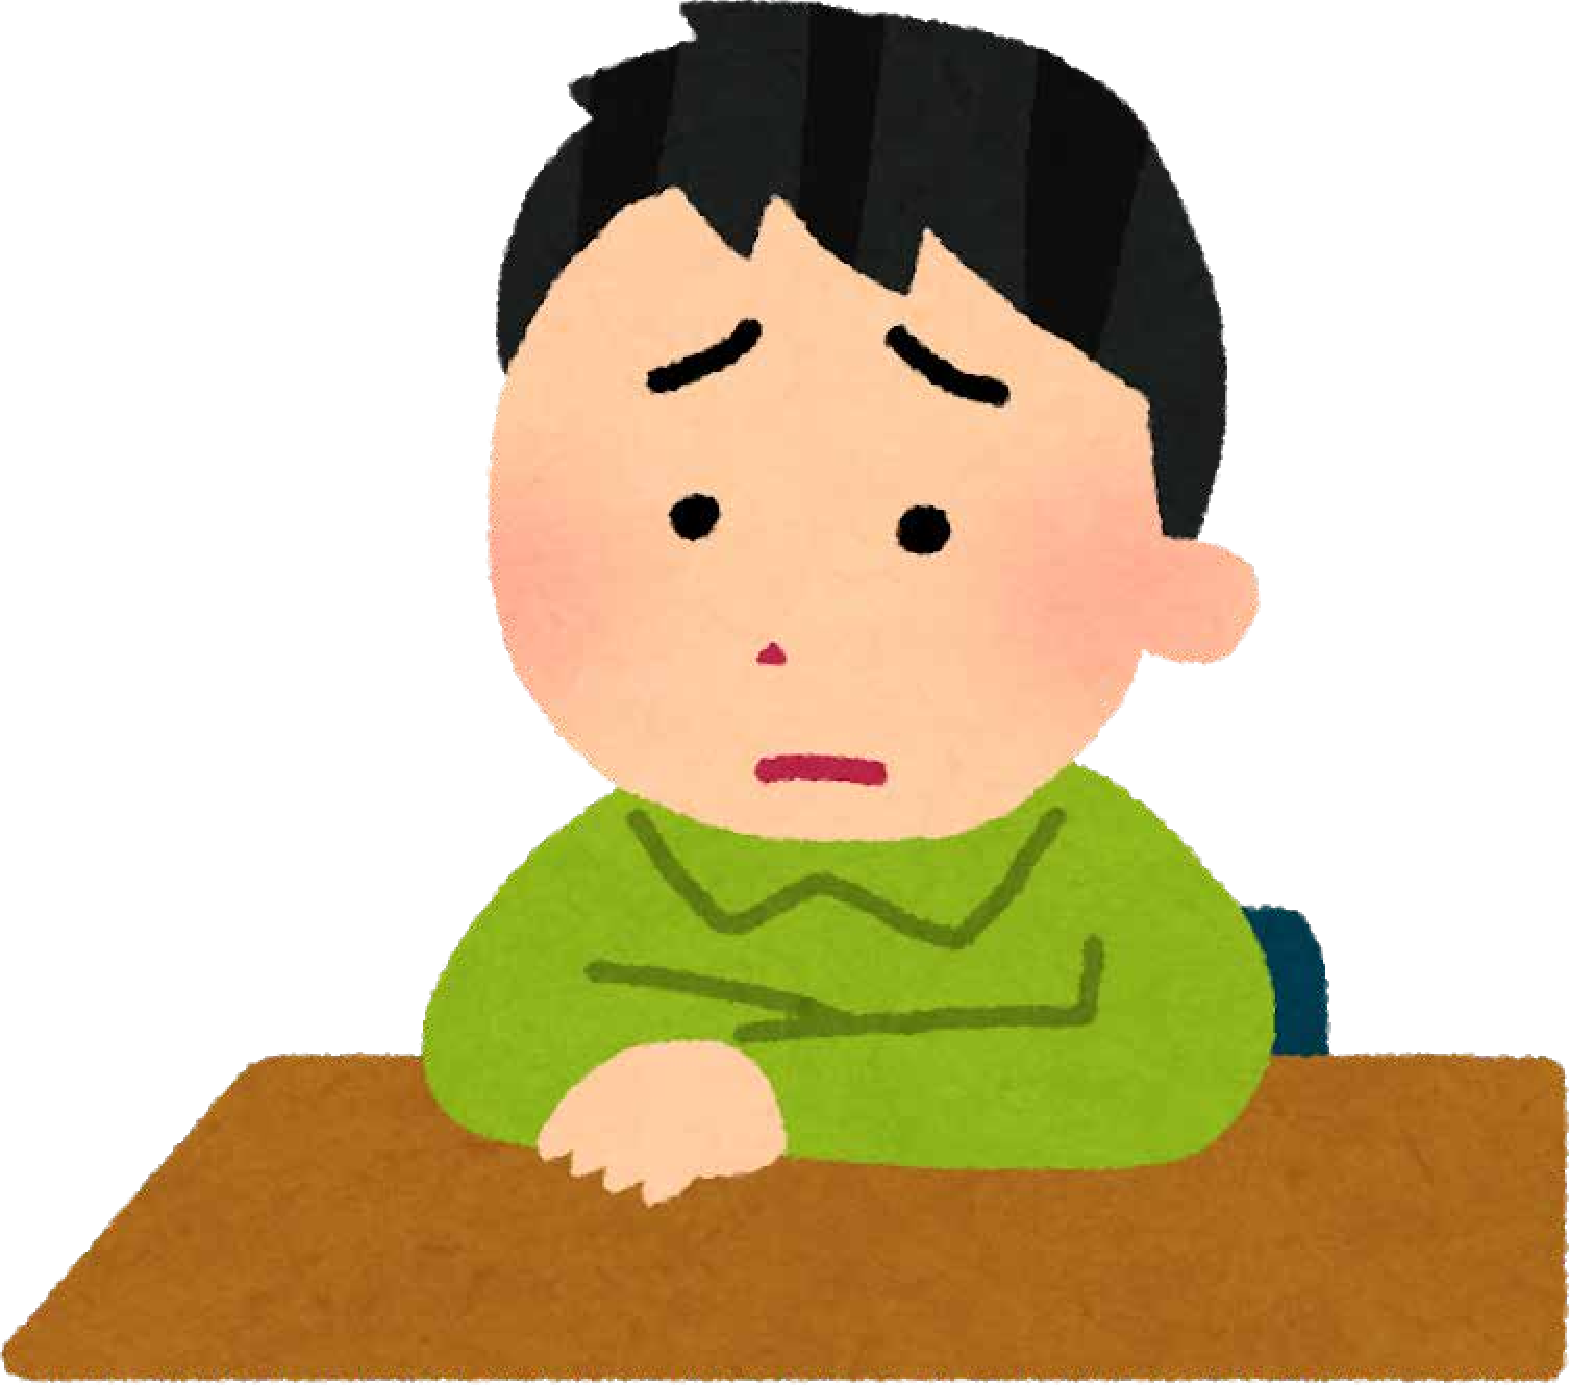
\includegraphics[width=\linewidth]{img/sample1.pdf}
  \caption{悩む男の子}
  \label{fig:sample1}
\end{figure}

\begin{figure*}[!tb]
  \centering
  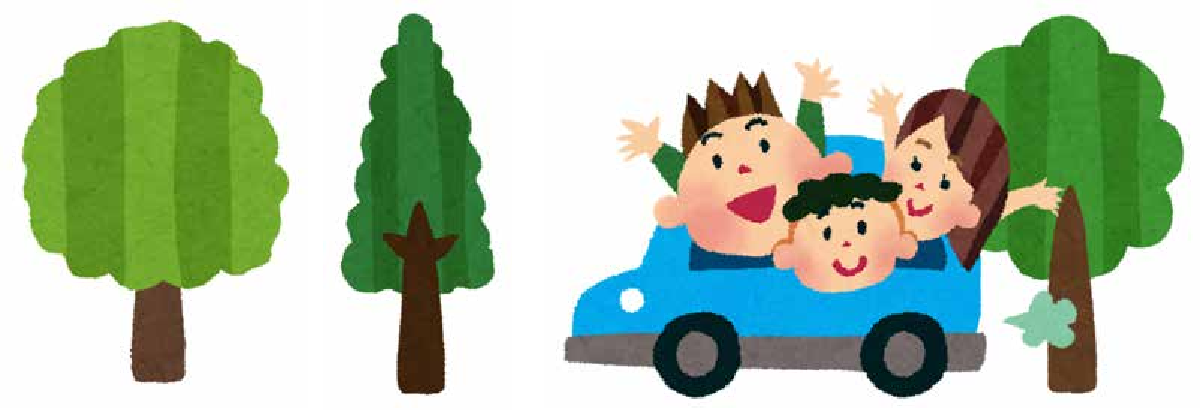
\includegraphics[width=\linewidth]{img/sample2.pdf}
  \caption{ドライブする家族}
  \label{fig:sample2}
\end{figure*}

%---------------------------------------------------------------------
\subsection{表}
表は\tabref{tab:data_type}のように引用することができ,表を作成する場合は罫線を少なくすることと,横線のみの使用を心がけることが推奨される.

\begin{table}[!bt]
  \caption{代表的なデータの型}
  \label{tab:data_type}
  \centering
  \begin{tabular}{lcr}
    \hline
    データの型         & 宣言   & ビット幅 \\
    \hline \hline
    短整数型           & short  & 16       \\
    整数型             & int    & 32       \\
    単精度浮動小数点型 & float  & 32       \\
    倍精度浮動小数店型 & double & 64       \\
    \hline
  \end{tabular}
\end{table}

%---------------------------------------------------------------------
\section{提案手法}

\begin{enumerate} % 箇条書きは \begin{itemize}
  \item 書かれた論文は書いた人の研究者としての人格を表す
  \item データのみ出して論文を書かない者は,テクニシャンである
  \item データも出さず,論文(原著論文)を書かない者は,評論家である
  \item 研究者は論文を書くことによって成長する.また,成長の糧にしなければならない
  \item 論文は研究者の飯のタネである
  \item 論文は後世の研究に影響を与えなければならない
  \item 研究者は書いた論文に責任を問われる
  \item 忙しくて論文が書けないというのは,言い訳にはならず,能力がないといっているのと同じである
  \item 博士論文以上の論文を書けない者は,その博士論文は指導教官のものといわれても仕方がない
  \item 研究において最も重要なのはアイデアであり,それが試されるのが論文である
\end{enumerate}

%---------------------------------------------------------------------
\section{評価}

%---------------------------------------------------------------------
\section{今後の課題}

%---------------------------------------------------------------------
% Bibliography
\footnotesize{
  \begin{thebibliography}{99}
    \bibitem{guideline} 総務省,帯域制御の運用基準に関するガイドライン(改定),2019.
    \bibitem{framework} Hung-Chin Jang and Jian-Ting Lin,SDN Based QoS Aware Bandwidth Management Framework of ISP for Smart Homes,
    \bibitem{latex_wiki} Latex Wiki (\url{https://texwiki.texjp.org/}).
    \bibitem{whats_paper} 渡辺 豊, "角皆静男先生のご逝去を悼む", 地球化学, vol.50, no.1, pp.1-3, 2016.
  \end{thebibliography}
}

%---------------------------------------------------------------------
\end{document}
%---------------------------------------------------------------------
